\textbf{\emph{Does our software application exhibit satisfactory user interface
efficiency and efficacy?}}

The application demonstrates good usability based on the results and
discussions presented in \Cref{sub:sus}. The SUS scores, as indicated by the
average of 80.3 and median of 85, reflect positive evaluations from the
participants. The SUS is a widely used questionnaire to measure usability, and
the high scores suggest that the participants found the application
user-friendly, intuitive, and easy to use.

Furthermore, the analysis of the SUS questionnaire's positive and negative
statements reveals that the participants generally agreed with the positive
statements, indicating their satisfaction with the application's usability.
Conversely, they disagreed with the negative statements, suggesting they did
not encounter significant usability issues or challenges while using the
application.

The positive evaluations and feedback from the participants regarding usability
provide strong evidence that the application is well designed and effectively
supports the monolith decomposition tasks.

\textbf{\emph{Does our software application contribute to the enhancement of
workload management and efficiency?}}

While looking at results obtained in Raw-TLX, \Cref{sub:raw-tlx}, the
participants rated the workload according to five categories: Mental Demand,
Temporal Demand, Performance, Effort and Frustration.

The usage of our application did not frustrate the participants, having an
average and median frustration of 3.33 and 3 points, respectively.

In regards to performance, the results are more balanced. Subjects did not feel
that the tool would have improved their decompositions, scoring an average of
5.27 and a median of 5. This result contradicts some results of \Cref{sub:sus}
and could be related to the fact that this question's positive answer shifted
to the left instead of keeping on the right. In fact, 27\% of the
participants that scored a SUS greater or equal to 70 answered as a 7 out of 10
regarding their success on the decomposition. This can be visualised in
\Cref{fig:sus_participant_performance} (for a better visualisation, Raw-TLX
Performance was scaled to match SUS scale).

\begin{figure*}[!htb]
  \caption{SUS vs Raw-TLX Performance}
  \label{fig:sus_participant_performance}
  \centering
  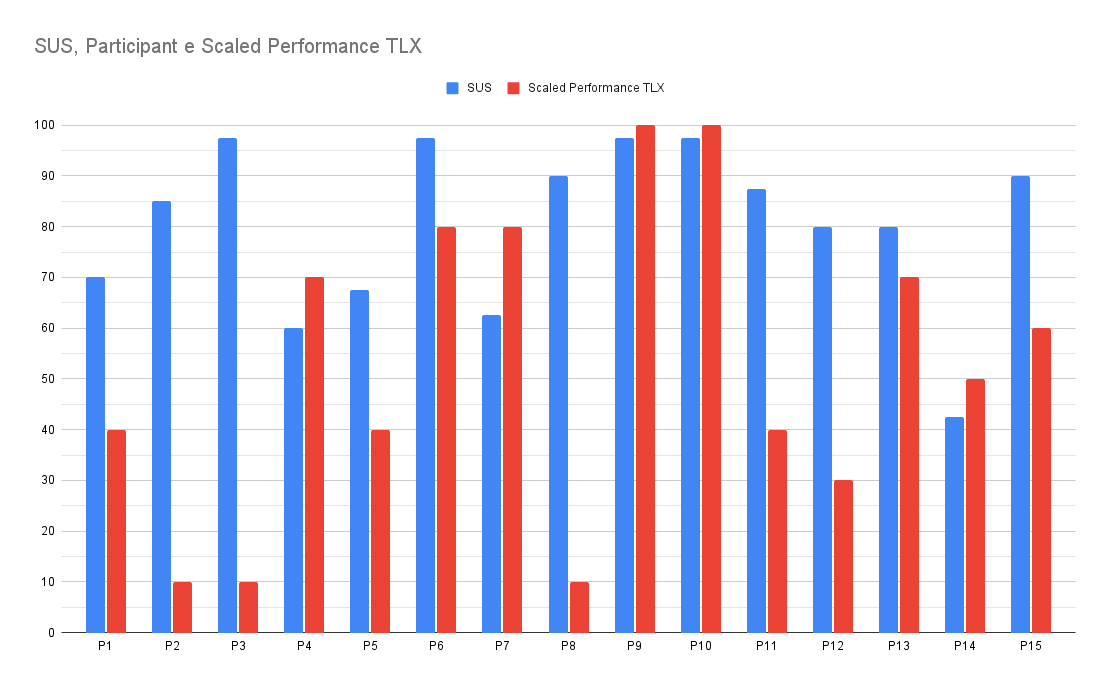
\includegraphics[width=\textwidth]{sus_participant_performace}
\end{figure*}

As for effort, subjects scored an average of 4.93 and a median of 5, which
means that the participants felt indifferent to how hard they had to work to
obtain their performance results.

The two demand levels score similarly, with 4 as the median and 4.40 4.47 for
mental and temporal demand, respectively. This means subjects did not find the
task mentally demanding or felt time pressure.

Overall, the application provided a mixed workload performance.

Despite the highly positive SUS scores, the Raw-TLX ratings were relatively
underwhelming. A possible explanation for this discrepancy is the absence of
contextual information provided during the task. Users relied solely on the
application to assist them in the decomposition process and encountered
particular challenges and frustrations, which may have resulted in slightly
negative sentiments. It would be beneficial to introduce a two-step approach to
address this issue. Initially, users could engage in a decomposition task
without utilising the application, followed by a subsequent task, using a
different project, involving employing the tool. This sequential methodology
has the potential to yield improved outcomes. Also, since decomposing a
monolith into microservices is a difficult task, not having something for
participants to compare the results to, may affect the perception on how much
the application helps them.
